\documentclass[tikz,dvipsnames]{standalone}
\usepackage{tikz-feynman}

\begin{document}

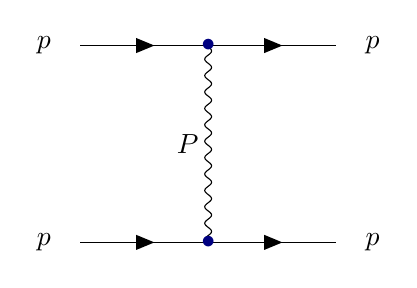
\begin{tikzpicture}
    \begin{feynman}

        \vertex (a){};

        \vertex[label=left:\(p\)] (i1) [left = 1.75cm of a]{};
        \vertex[label=right:\(p\)] (i2) [right = 1.75cm of a]{};

        
        \vertex (b) [below= 2.5cm of a]{};

        \vertex[label=left:\(p\)] (i3) [left= 1.75cm of b]{};
        \vertex[label=right:\(p\)] (i4) [right= 1.75cm of b] {};
;

        \diagram*{
        (i1) -- [fermion] (a.center)-- [fermion] (i2),

        (a.center) --[boson, edge label'=\(\mathbb{P}\)] (b.center),
        
        (i3) -- [fermion] (b.center)-- [fermion] (i4) };
    \end{feynman}

\node at (a) {\textcolor{NavyBlue}{$\bullet$}};
\node at (b) {\textcolor{NavyBlue}{$\bullet$}};
\end{tikzpicture}

\end{document}